% fancytikzposter.tex, version 2.1
% Original template created by Elena Botoeva [botoeva@inf.unibz.it], June 2012
% 
% This file is distributed under the Creative Commons Attribution-NonCommercial 2.0
% Generic (CC BY-NC 2.0) license
% http://creativecommons.org/licenses/by-nc/2.0/ 
\documentclass{a0poster}
\usepackage[USenglish]{babel}% or british
\usepackage[T1]{fontenc}


\usepackage{wrapfig}
\usepackage{fancytikzposterM} 
\usepackage{multirow}
\usepackage{array}

% background picture
\usebackgroundtemplate{7}

\definecolor{myblue3}{HTML}{0C3E07}%main frames


\usepackage[margin=\margin cm, paperwidth=84.1cm, paperheight=118.9cm]{geometry}


\usepackage{cmbright}
%\usepackage[default]{cantarell}
%\usepackage{avant}
%\usepackage[math]{iwona}
\usepackage[math]{kurier}
\usepackage[T1]{fontenc}
\usepackage{tikz}

%%%%%%%%%%%%%%%%%%%%%%%%%%
%%% SET FONT SIZES %%%%%%%%%%%%%
%%%%%%%%%%%%%%%%%%%%%%%%%%
\renewcommand{\Huge}{\fontsize{64}{85}\selectfont} % Main title
\renewcommand{\huge}{\fontsize{44}{70}\selectfont} % Sub title
\renewcommand{\LARGE}{\fontsize{48}{48}\selectfont} % Box headers
\renewcommand{\Large}{\fontsize{42}{40}\selectfont} % Authors
\renewcommand{\normalsize}{\fontsize{40}{42}\selectfont} % Text in the boxes
\renewcommand{\footnotesize}{\fontsize{34}{42}\selectfont} % references
\renewcommand{\small}{\fontsize{24}{22}\selectfont}
%% add your packages here


%% Set the folder that contains the images
\graphicspath{ {./Lowres/} }


\title{Genetic evolution, climate change, and wild vertebrates extinction: predicting and caring\vspace{-0.2em}}
\author{{\LARGE{Dr. Timoth\'{e}e Bonnet}}\\ \vspace{-20pt} \footnotesize Research School of Biology, ANU College of Science
\\
}

\begin{document}

%%%%% ---------- the background picture ---------- %%%%%
%% to change it modify the macro \BackgroundPicture
\ClearShipoutPicture
\AddToShipoutPicture{\BackgroundPicture}

\noindent % to have the picture right in the center

\begin{tikzpicture}
  \initializesizeandshifts
  % \setxshift{15}
  \setyshift{2.5} % uncomment this line to condense the boxes

  \newcommand{\volesize}{0.8cm}

  %% the title block, #1 - shift, the default value is (0,0), #2 - width, #3 - scale
  %% the alias of the title block is `title', so we can refer to its boundaries later
  \ifthenelse{\equal{\template}{1}}{ 
    \titleblock[(-0.7,0)]{48}{1}
			}{
    \titleblock[(-10,0)]{87}{1.5}
			}
			
\addlogo[east]{(10,0)}{8cm}{anu}
\addlogo[west]{(-10,0)}{8cm}{tim}

\coordinate (aaa) at (currenty);

	\blocknodew[($(currenty)+(19.6,0)$)]{77}{(
\includegraphics[width=\volesize]{snowwwvole2}) Human activities modify the environment of many wild animals,\dots}
		{
		   \dots threatening animal populations, and changing selective pressures. Lab experiments have shown that genetic evolution can be fast enough to rescue populations from extinction, but in nature, we know close to nothing about how and when evolution makes a difference. There are three main problems: (
\includegraphics[width=\volesize]{snowwwvole2}) Population monitoring are too short and not detailed enough; (
\includegraphics[width=\volesize]{snowwwvole2}
\includegraphics[width=\volesize]{snowwwvole2}) Adaptive evolution is impossible to demonstrate without genetic data (expensive) and genetic models (complicated); (
\includegraphics[width=\volesize]{snowwwvole2}
\includegraphics[width=\volesize]{snowwwvole2}
\includegraphics[width=\volesize]{snowwwvole2}) A lack of tools to jointly model genes and demography. How to tackle these challenges? \vspace{-0.8cm}
		}
	
%%%%%%%%%%%%%%%%%%%%%%%%%%%%%%%%%%%%%%%%%%%%%%%%%%%%%%%%%%%%%%%%%%%%%%%%%%%%%	
	\blocknodew[($(currenty)+(0,2)$)]{77}{(
\includegraphics[width=\volesize]{snowwwvole2}
\includegraphics[width=\volesize]{snowwwvole2}) To understand and predict how wild population respond to environmental change, we need\dots}
	{
	\hspace{-1cm}
		\begin{tabular}{p{0.25\textwidth} p{0.03\textwidth} p{0.22\textwidth} p{0.03\textwidth} p{0.22\textwidth} p{0.25\textwidth}}
		
		\parbox{22cm}{Long-term monitoring in the wild\\
		  \centering  \begin{tabular}{c c}
		      \includegraphics[height=12cm]{DSC00190}  & 
		      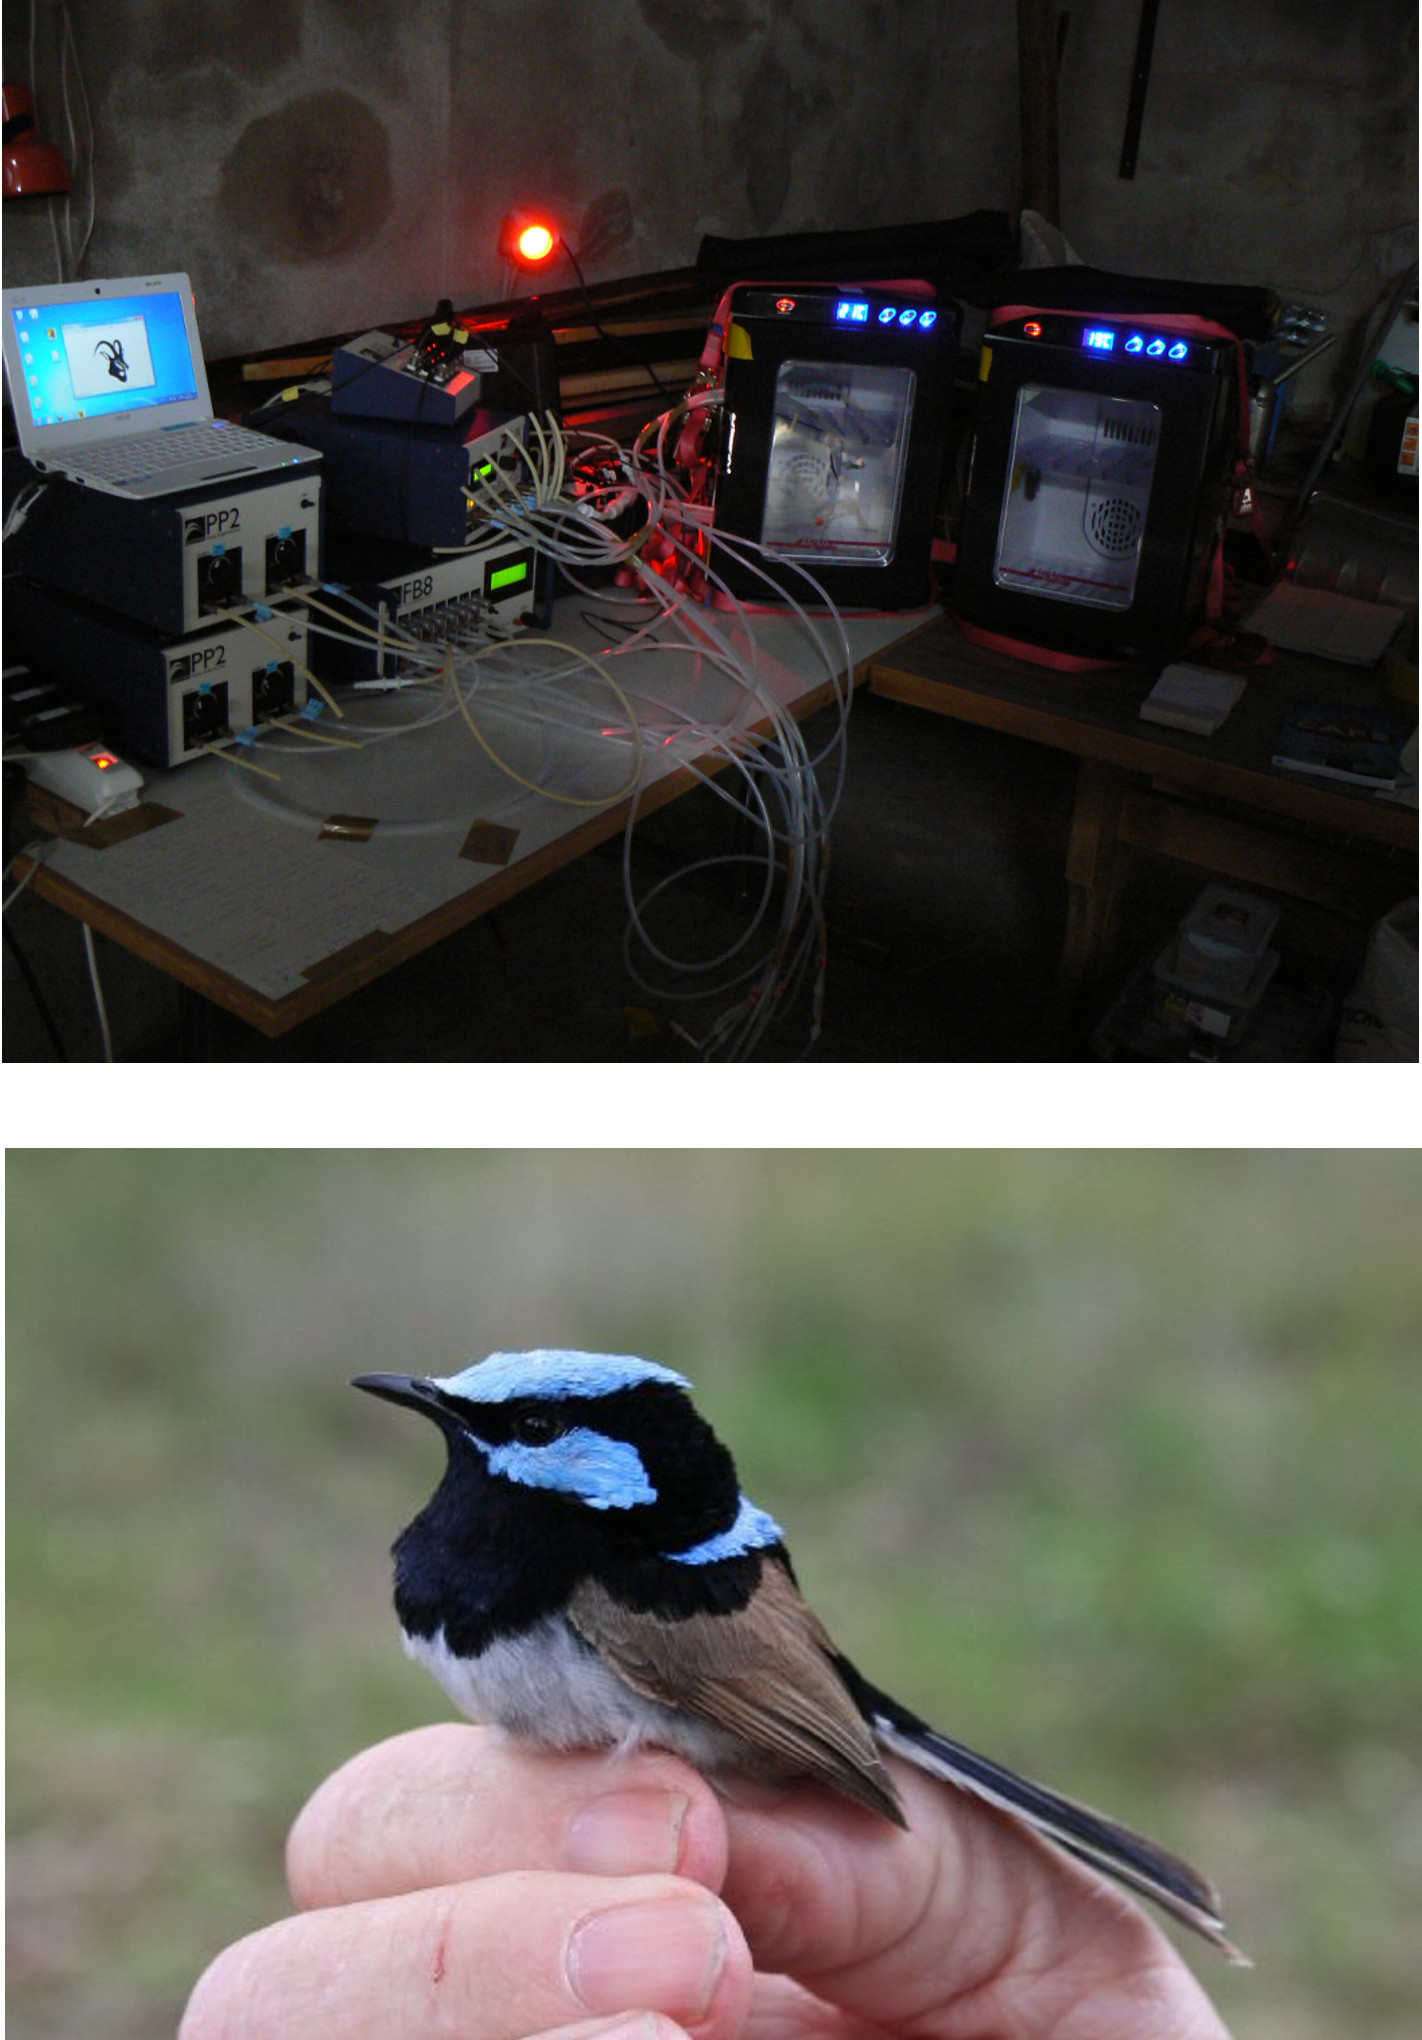
\includegraphics[height=12cm]{field} \\
		    \end{tabular}
		  }
		  &
		  &
		\parbox{20cm}{ \hspace{4cm}Weather data\\
		   \centering \begin{tabular}{c}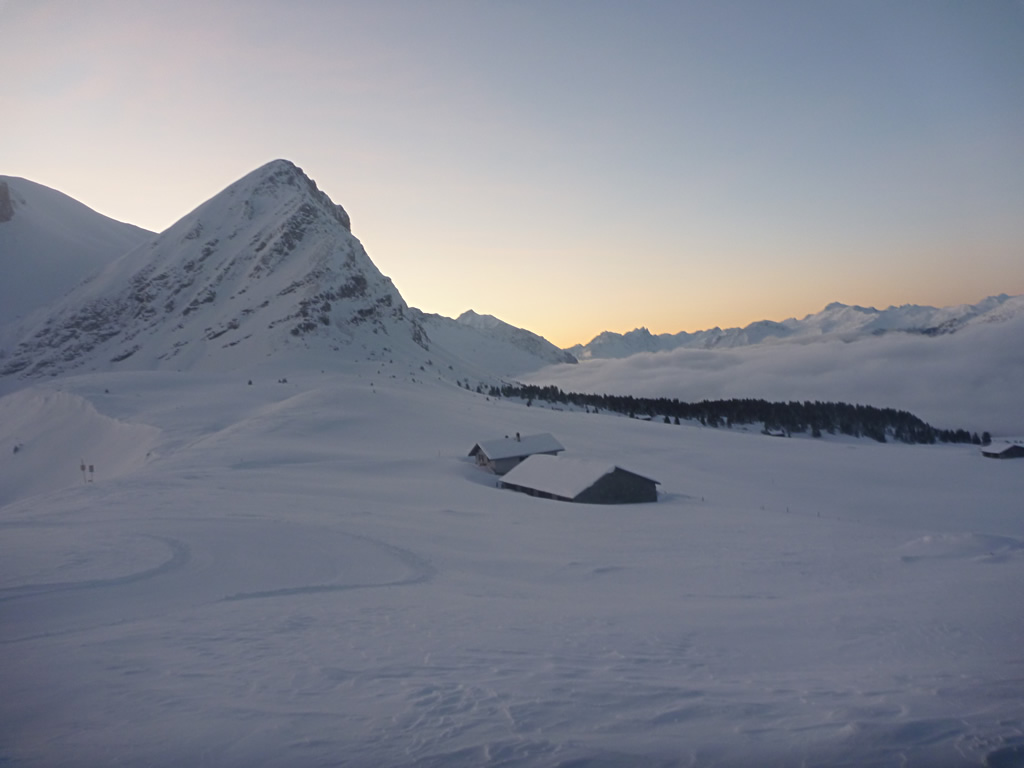
\includegraphics[height=12cm]{Taliflue-winter}\end{tabular}
		  }
				&
				&
		\parbox{20cm}{ Genetic / genomic data\\
		\centering \begin{tabular}{c} 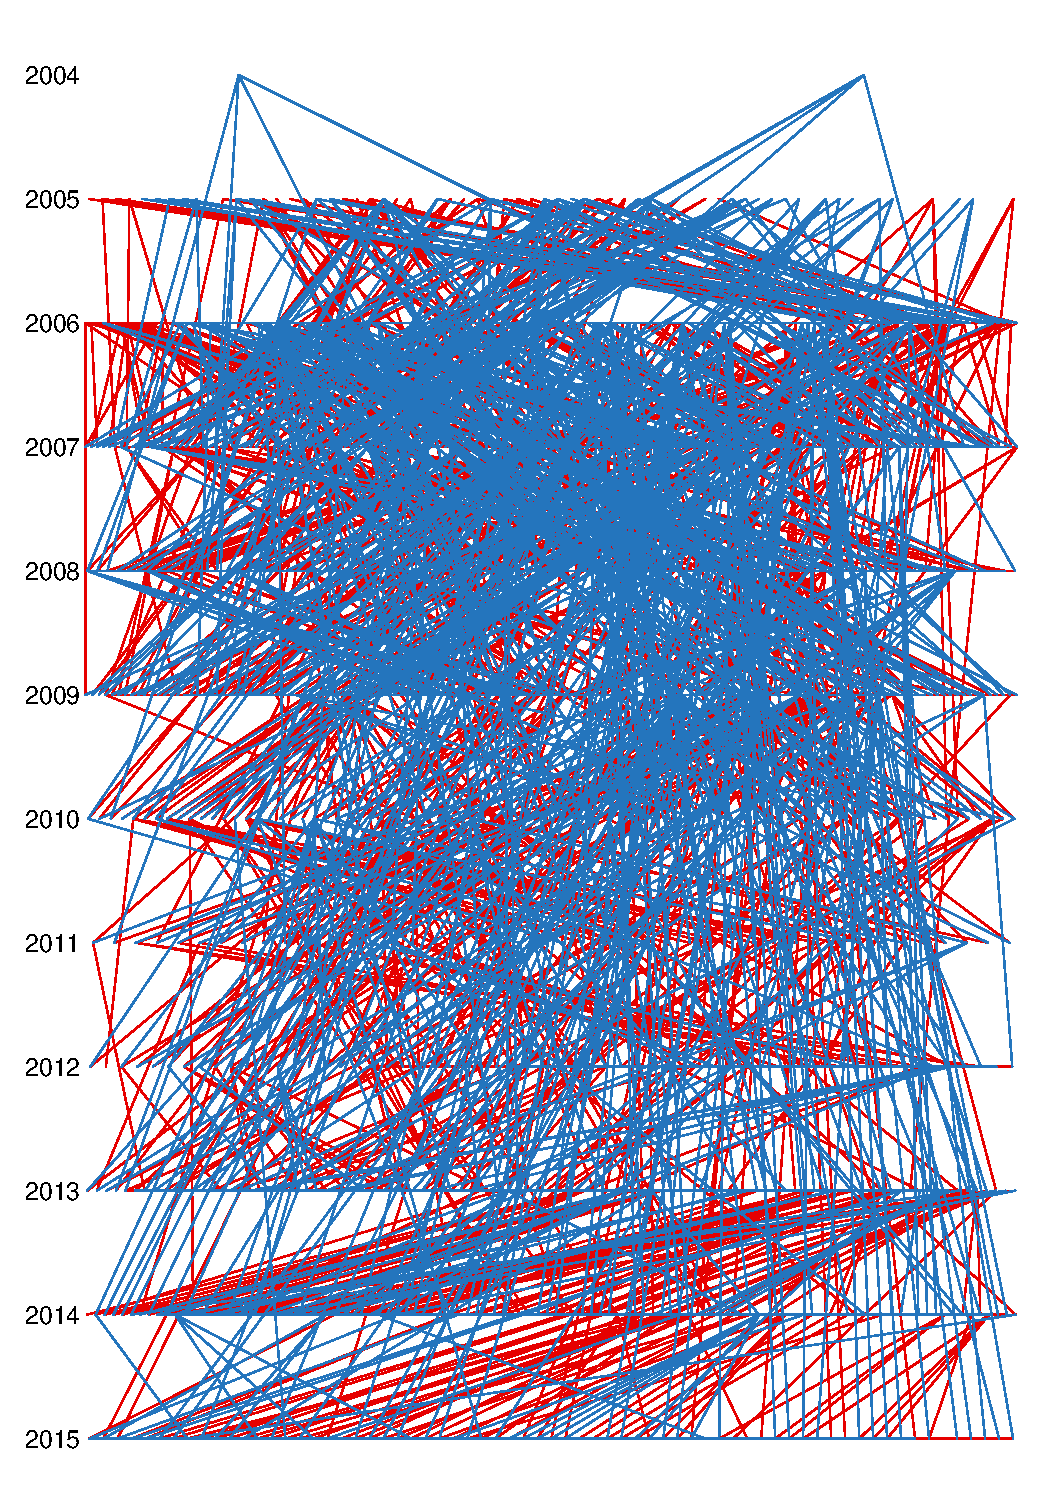
\includegraphics[height=12cm]{pedigreeplot}\end{tabular}
		  }
				&
		\parbox{20cm}{\hspace{1cm}Math/statistical tools\\
		 \centering \begin{tabular}{c} 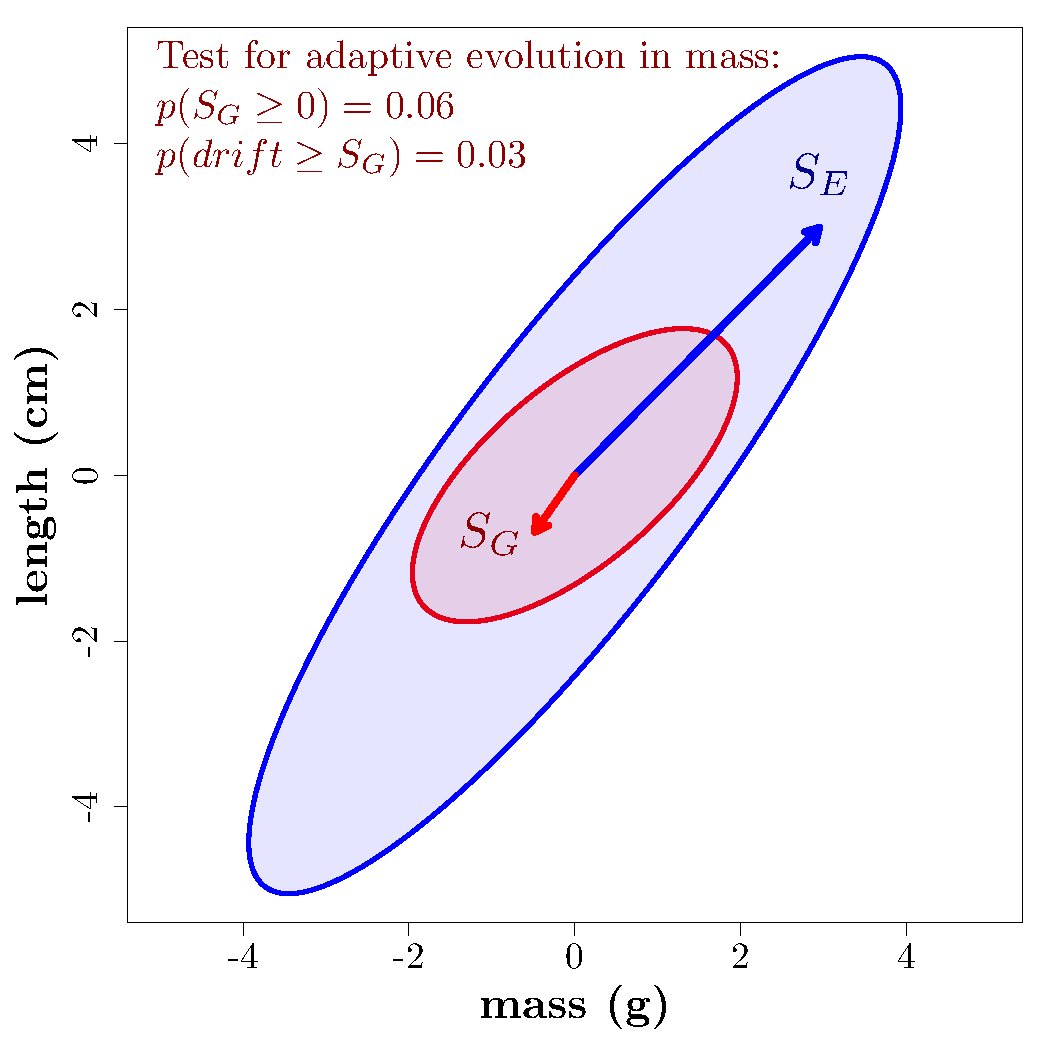
\includegraphics[height=12cm]{Matrices-1}\end{tabular}
		  }	
		\end{tabular}
		\vspace{-1cm}
	}%end block
%%%%%%%%%%%%%%%%%%%%%%%%%%%%%%%%%%%%%%%%%%%%%%%%%%%%%%%%%%%%%%%%%%%%%%%%%%%%%	
	\coordinate (tfirstcol) at (currenty);
	
 \coordinate (width) at ($(76.8,0) - (2.1,0)$);   
 %% the content of the block
  %% the content of the block
          \draw let \p1=($(width)-(0,0)$) , \p2=($(0,\blocktitleheight cm)-(0,2.4cm)$)
          in node[draw, anchor=north, color=blocktitlefillcolor, text=blocktextcolor, 
          frame, rectanglesplittwo, rectangle split horizontal=false, 
          rectangle split part fill={blocktitlefillcolor, none}, %
          rectangle split empty part height= \y2 
          ]
          (box) at ($(currenty)+(0,2)$) {
            \nodepart{second}
            \begin{minipage}{\x1}
            \begin{center}
	      \vspace{22cm} % a very mesy trick to control box height...
            \end{center}
           \end{minipage}
          }; 

          %% the title of the block
          \node[frame, anchor=north west, text=blocktitletextcolor] at (box.north west)
          {(
\includegraphics[width=\volesize]{snowwwvole2}
\includegraphics[width=\volesize]{snowwwvole2}
\includegraphics[width=\volesize]{snowwwvole2}) \bf\LARGE Measuring and predicting genetic adaptation to environmental changes };  
          
          \node[anchor=north west] (deer) at ($(box.north west)+(0.2,-3)$) {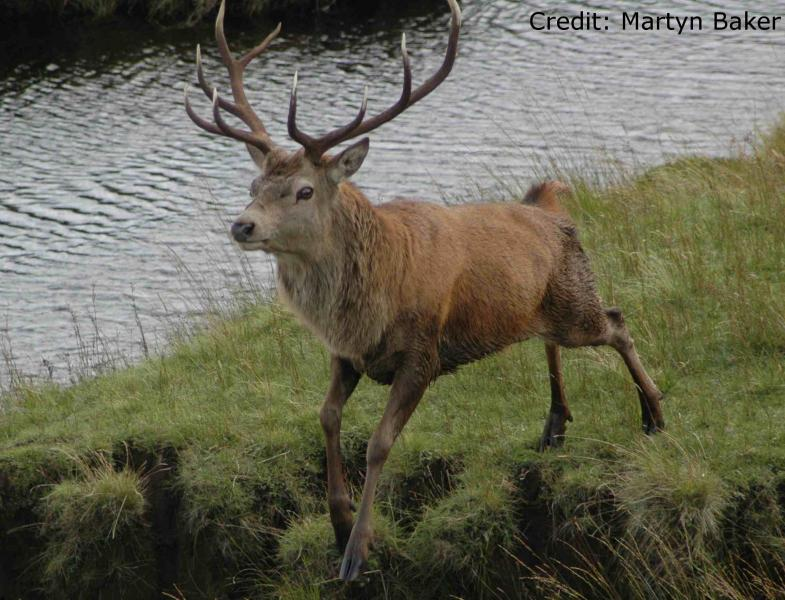
\includegraphics[height=10cm]{percy}};
          \node[anchor=south] (reddeer) at (deer.south) {\color{colorone!40!white}{\large Red deer, Scotland}};
          \node[anchor=west] (clim1) at (deer.east) {\parbox{10cm}{\textbf{Earlier, warmer springs affect parturition date}}};
          
          
          \node[anchor=south west] (vole) at ($(box.south west)+(0.2,3)$) {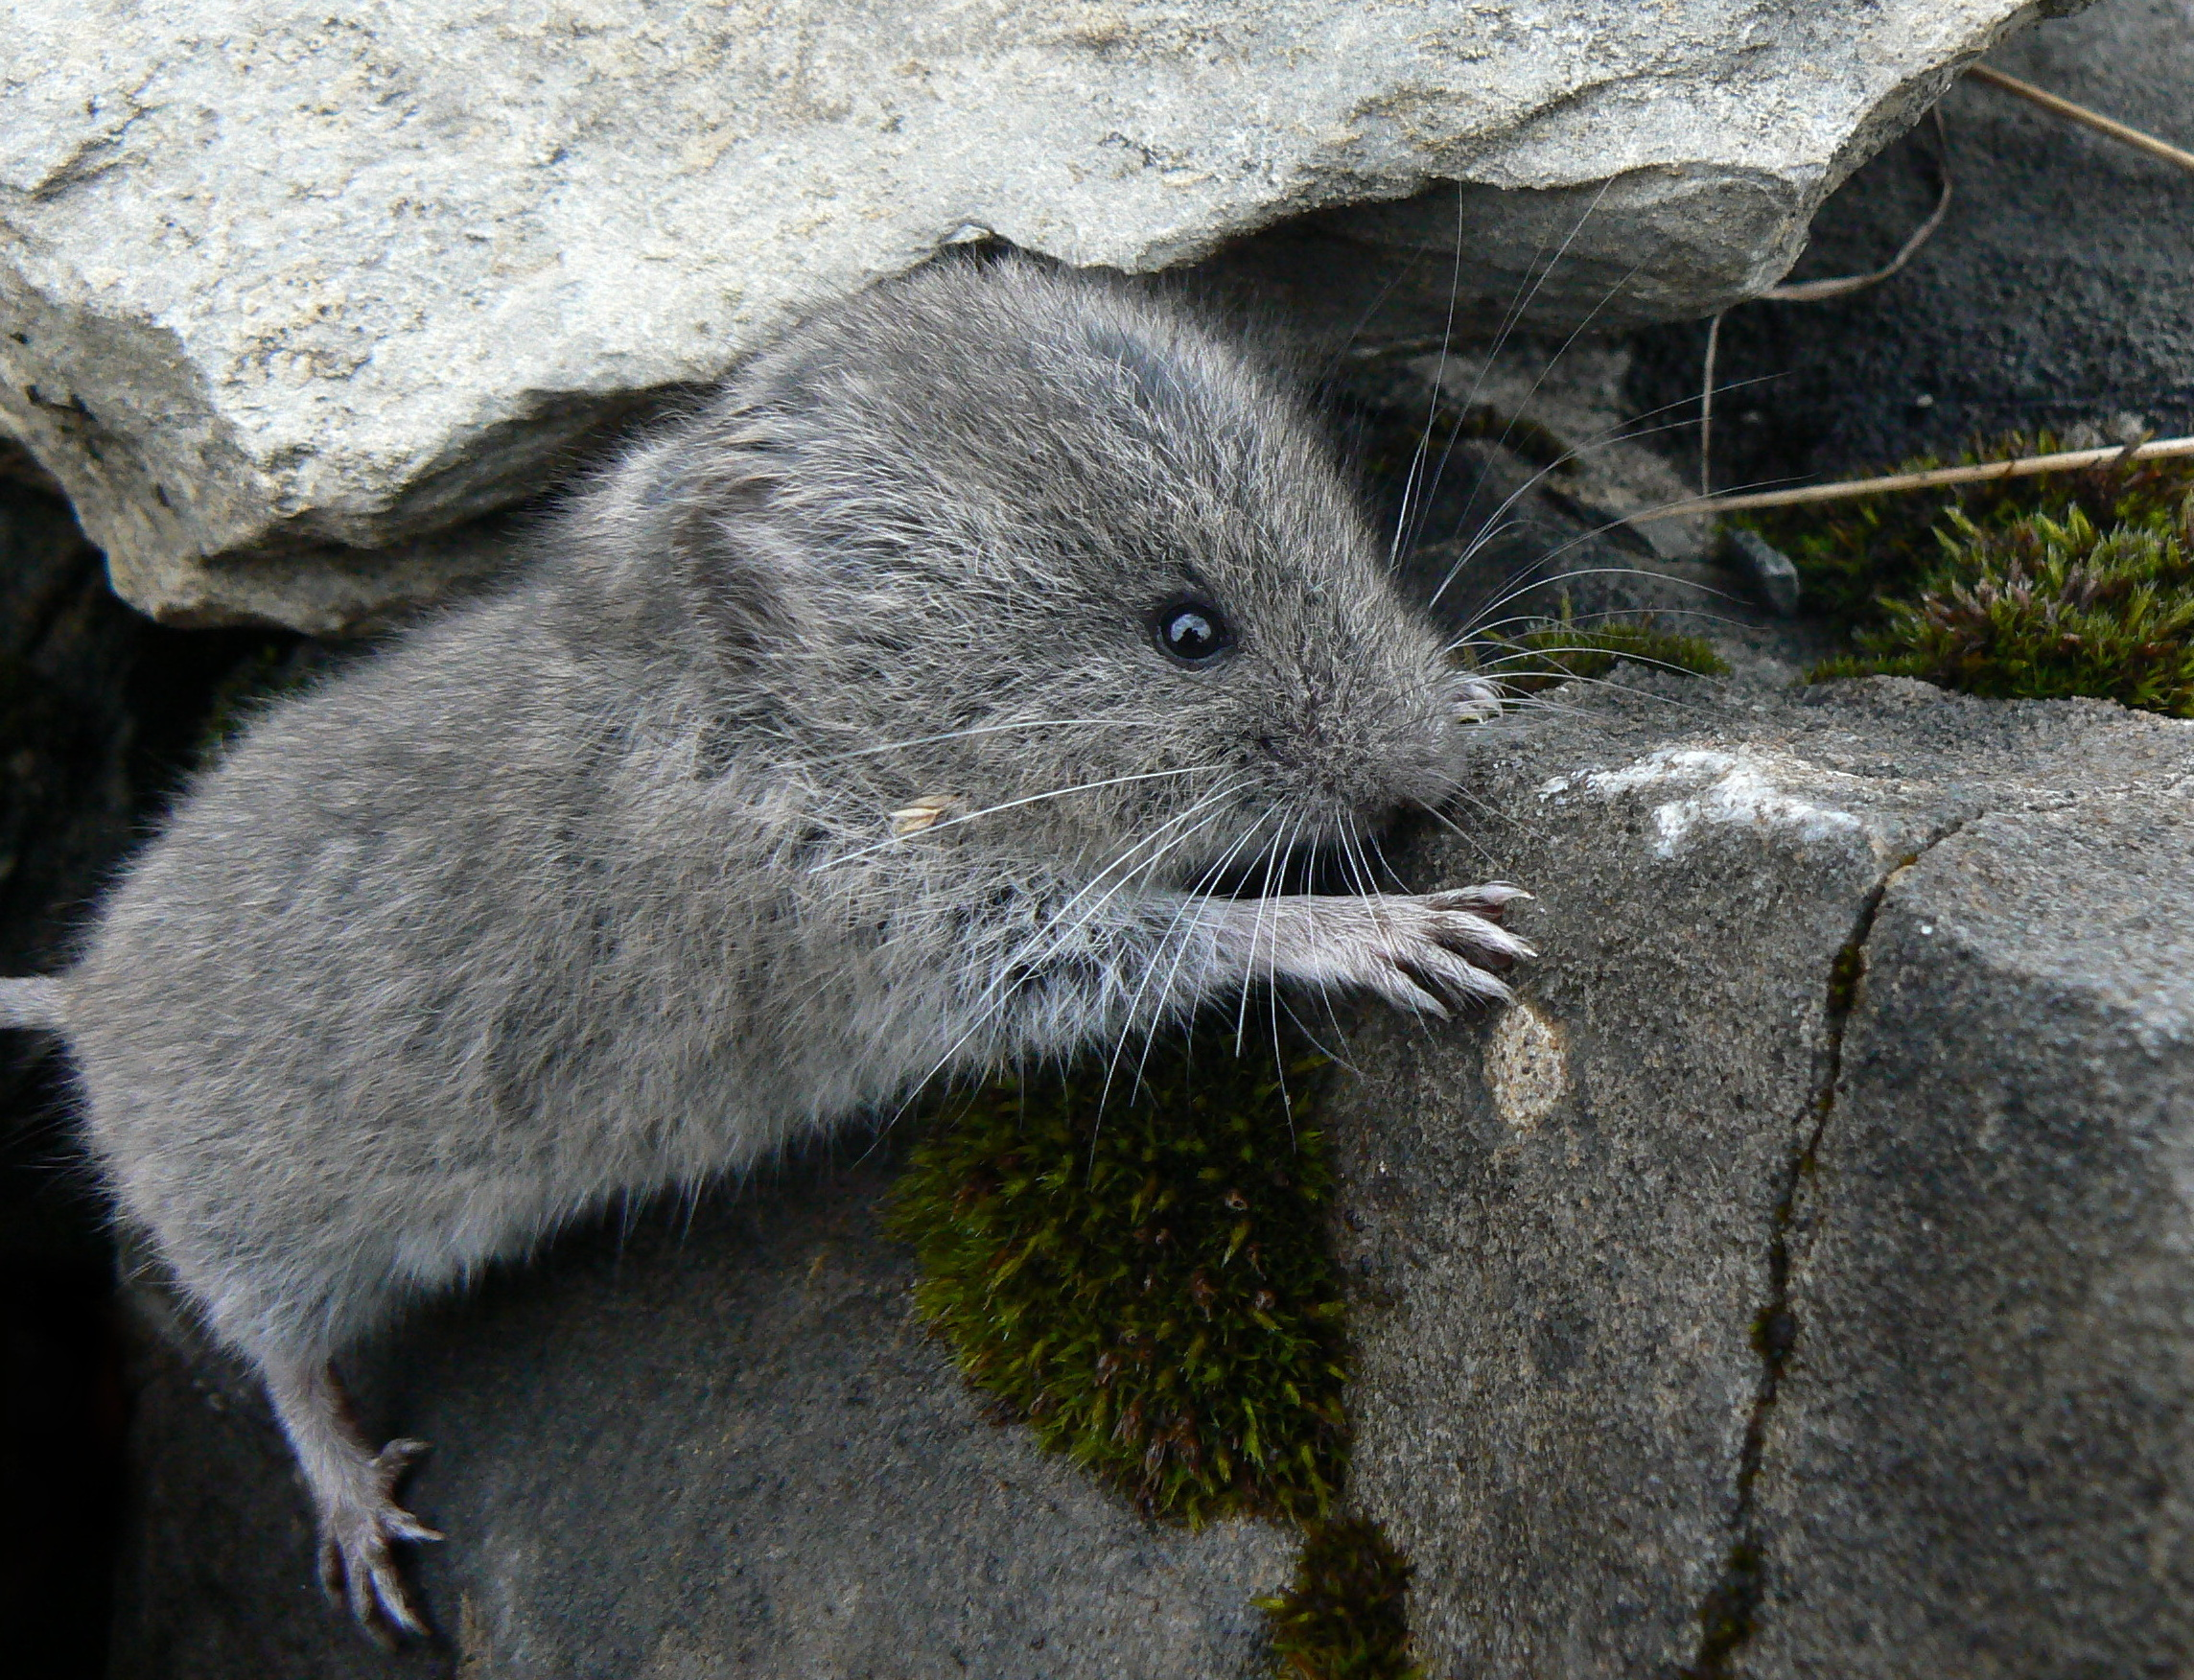
\includegraphics[height=10cm]{cutevole}};
          \node[anchor=south] (snowvole) at (vole.south) {\color{colorone!40!white}{\large Snow vole, Switzerland}};

          \node[anchor=west] (clim2) at (vole.east) {\parbox{10cm}{\textbf{Change in snow fall pattern affect body mass}}};
          
          \node[anchor=west] (graph) at ($(box.west)+(20.5,-1)$) {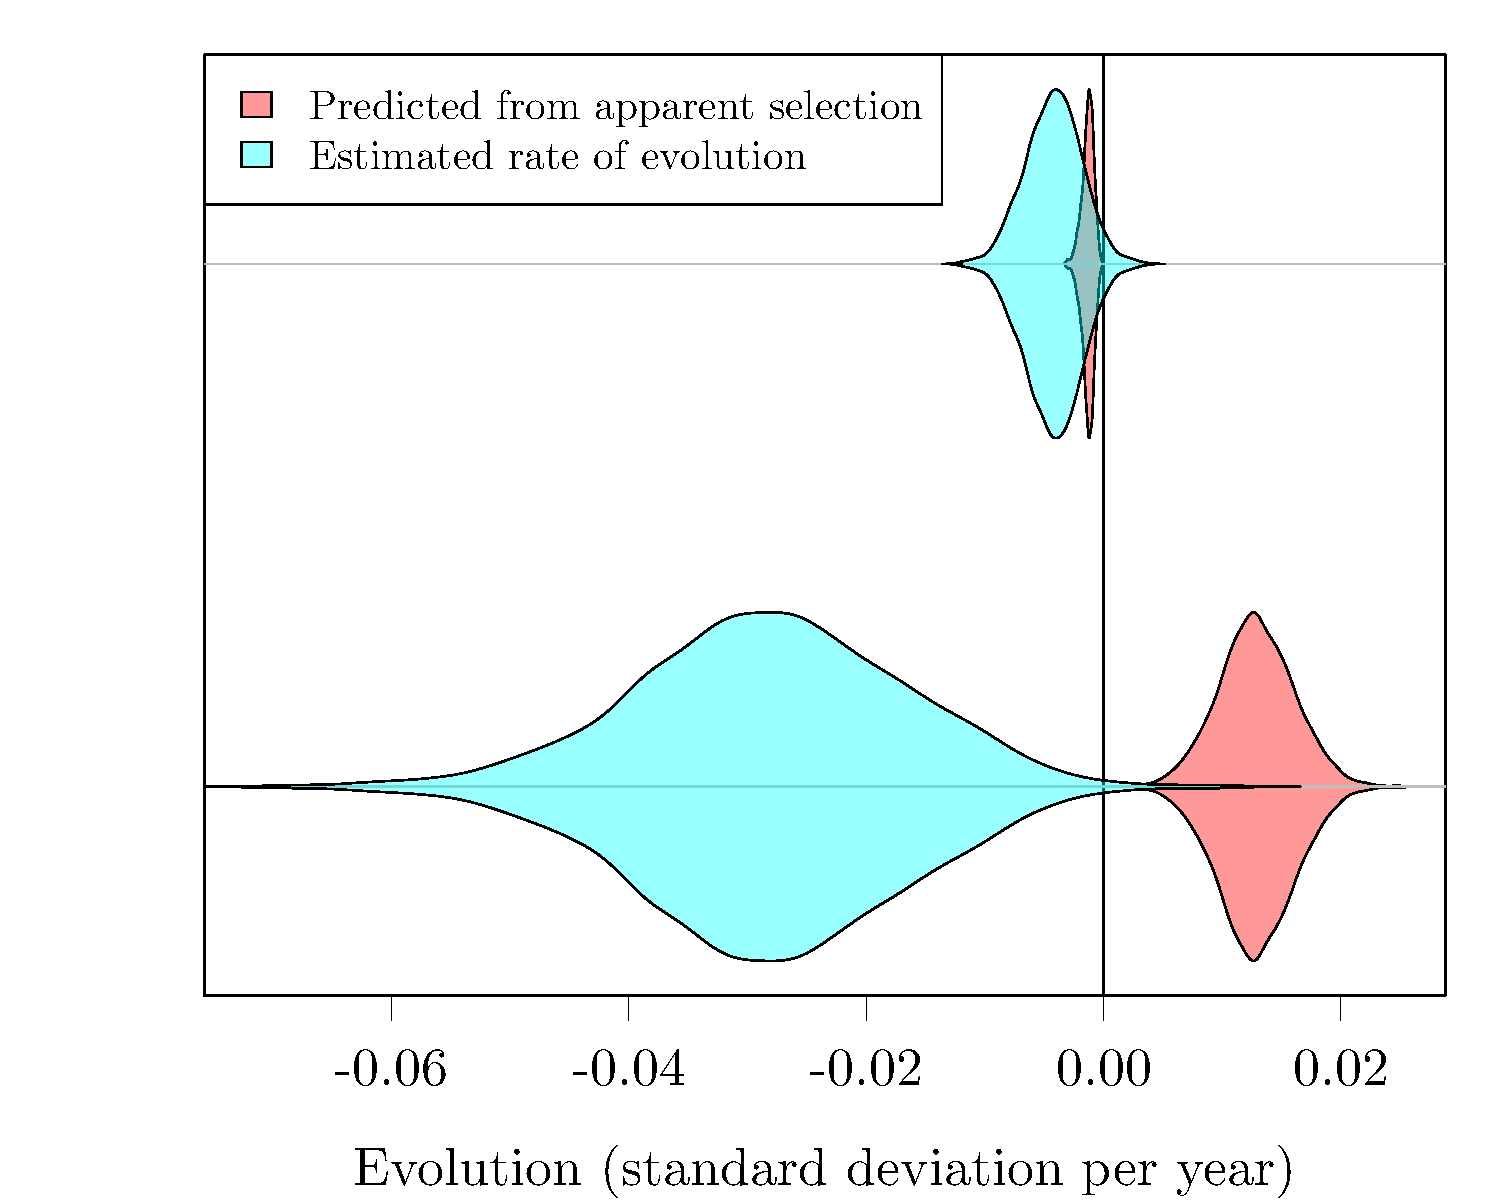
\includegraphics[height=25cm]{MakeGraph/figure/gr-1}};
                
           \node[anchor=east] (evolcommon) at ($(box.east)+(-0.5,3.5)$) {\parbox{24cm}{\textbf{Statistical partitioning of phenotype reveals rapid genetic change.\\
           \\Apparent selection may not predict evolution well.\\
           \\Phenotypic data are necessary but insufficient to predict evolution}}};
                    
	  \node[anchor=south east,  draw=colorone!70!black] (text1) at ($(box.south east)+(-0.5,3)$) {\parbox{24cm}{\textbf{\color{colorone!70!black}{Genetic evolution over a few generations, related to climate change.\\ \textit{How common is it?}}}}};
	  
   \coordinate (currenty) at ($(box.south)-(yshift)$);
%%%%%%%%%%%%%%%%%%%%%%%%%%%%%%%%%%%%%%%%%%%%%%%%%%%%%
          \draw let \p1=($(width)-(0,0)$) , \p2=($(0,\blocktitleheight cm)-(0,2.4cm)$)
          in node[draw, anchor=north, color=blocktitlefillcolor, text=blocktextcolor, 
          frame, rectanglesplittwo, rectangle split horizontal=false, 
          rectangle split part fill={blocktitlefillcolor, none}, %
          rectangle split empty part height= \y2 
          ]
          (box2) at ($(currenty)+(0,2)$) {
            \nodepart{second}
            \begin{minipage}{\x1}
            \begin{center}
	      \vspace{22cm} % a very mesy trick to control box height...
            \end{center}
           \end{minipage}
          }; 
          
                    %% the title of the block
          \node[frame, anchor=north west, text=blocktitletextcolor] (tit2) at (box2.north west)
          {(
\includegraphics[width=\volesize]{snowwwvole2}
\includegraphics[width=\volesize]{snowwwvole2}
\includegraphics[width=\volesize]{snowwwvole2}
\includegraphics[width=\volesize]{snowwwvole2}) \bf\LARGE Understanding the interplay between genetic evolution and population dynamics}; 

          
          \node[anchor=north] (evolution) at ($(box2.north)+(0,-3)$) {\textbf{\LARGE Evolution}};
          \node[anchor=south] (demography) at ($(box2.south)+(0,0)$) {\textbf{\LARGE Demography}};
	  
	  \draw[->, line width=0.4cm, color = colorone!70!black] ($(evolution.south)-(0.5,1)$) -- ($(demography.north)-(0.5,0)$);
	  \draw[<-, line width=0.4cm, color = colorone!95!white] ($(evolution.south)+(0.5,0)$) -- ($(demography.north)+(0.5,1)$);
          
          \node[anchor=east, draw=colorone!70!black] (rescue) at ($(box2.west)+(38,0)$) {\parbox{16cm}{\color{colorone!70!black}{\textbf{\textit{How fast can adaptation up-bend population growth rate? When?}}}}};
          
          \node[anchor=north west] (demoevo) at ($(box2.north west)+(1,-3)$) {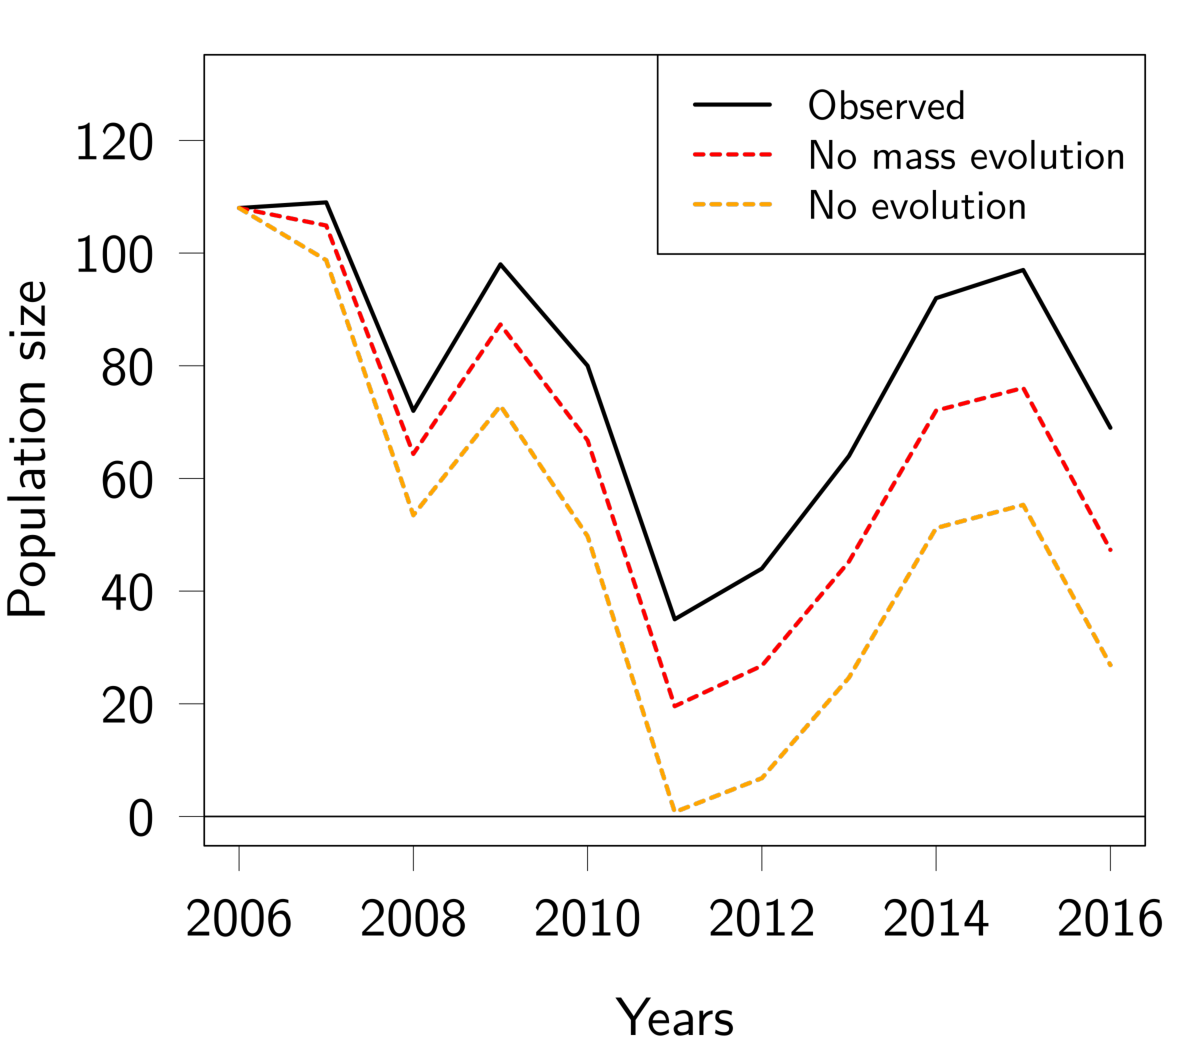
\includegraphics[width=18cm]{projnoevolevolmass-1}};
          

          
          \node[anchor=west, draw=colorone!95!white] (oppsel) at ($(box2.west)+(39,0)$) {\parbox{16cm}{\color{colorone!95!white}{\textbf{\textit{Does the opportunity for selection increase when populations crash?}}}}};
          
          \node[anchor=north east] (reiss) at ($(box2.north east)+(0,-5)$) {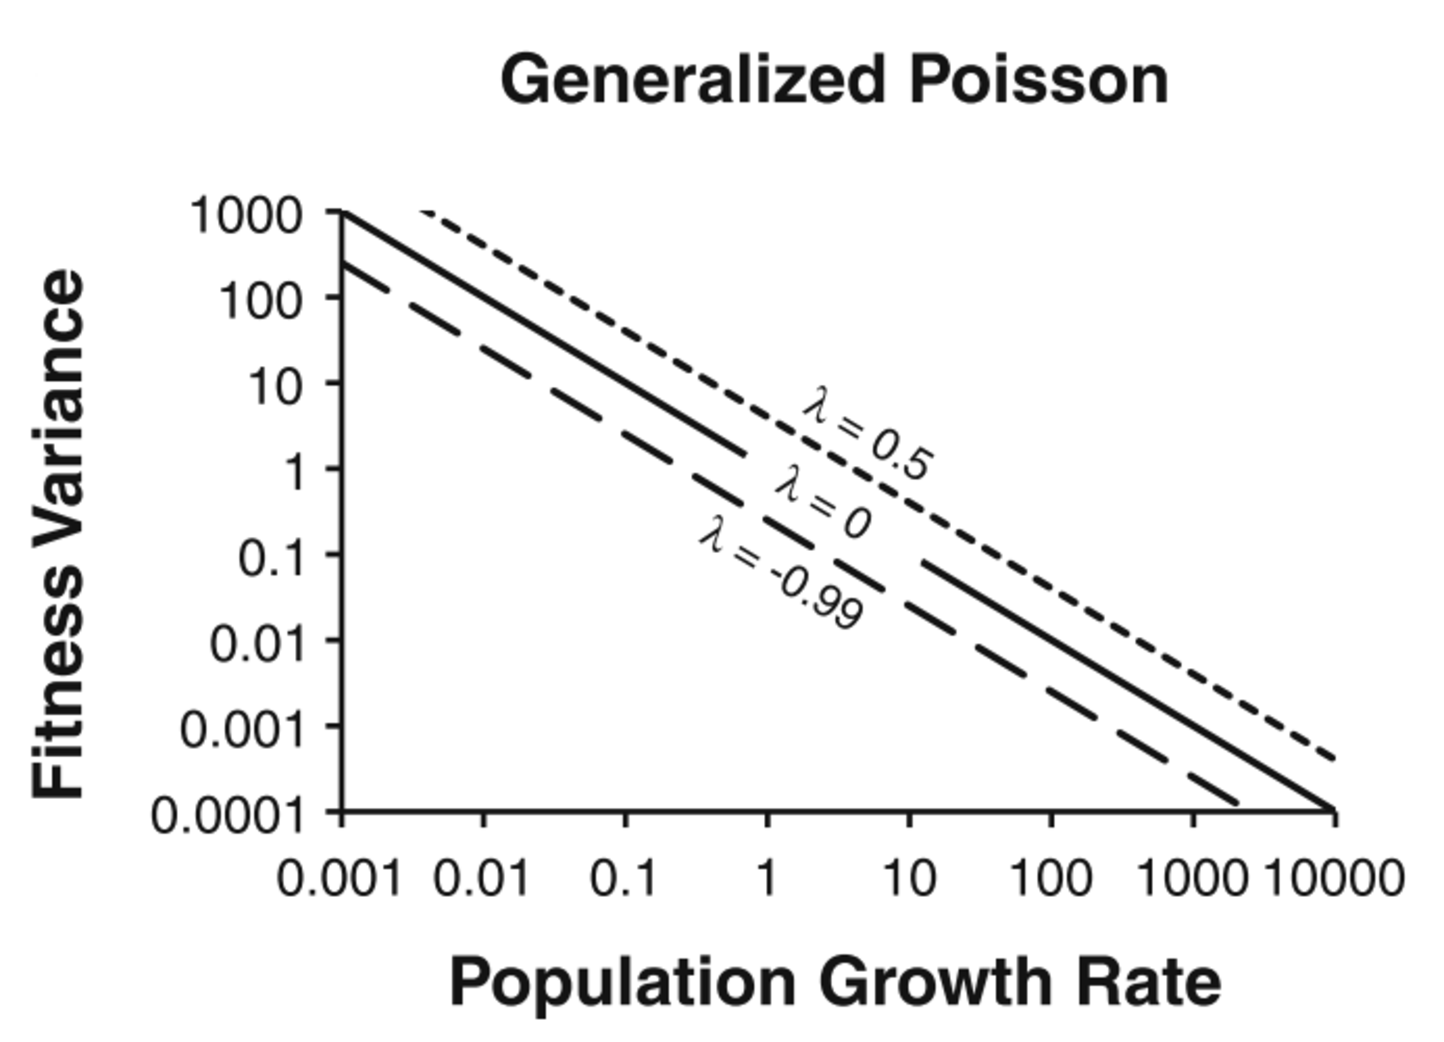
\includegraphics[width=20cm]{reissexpected}};
          
          %\node[anchor=south east] (theory) at ($(box2.north east)+(-1,-6)$) {};
          \node[anchor=south east, draw=black] (metaana) at ($(box2.south east)+(-0.5,2)$) {\parbox{32cm}{Theoretical expectation\\But relies on mathematical models \\ \textbf{Meta-analysis to confirm pattern empirically}}};
          
          \node[anchor=south west, draw=black] (demograph) at ($(box2.south west)+(0.5,2)$) {\parbox{32cm}{Evolution can rescue populations\\ Cannot be sure without knowing nature of selection\\ \textbf{Needs long(er)-term data}}};
          
 %%%%%%%%%%%%%%%%%%%%%%%%%%%%%%%%%%%%%%%%%%%%%%%%%%%%%%%%%%%%%%%%%%%%%%%%%%%%%%%
   \coordinate (currenty) at ($(box2.south)-(yshift)$);

    \node[anchor=north, rounded corners=15pt, fill=titledrawcolor] (qrw) at ($(currenty) + (-34,0)$) {
\includegraphics[width=8cm]{qrwebsite}};
    \node[anchor=north, rounded corners=15pt, fill=titledrawcolor] (qrgit) at ($(currenty) + (34,0)$) {
\includegraphics[width=8cm]{qrgitrepos}};
    \node[anchor=south] (web) at (qrw.north) {\textbf{\color{colorone!80!black}{Website}}};
    \node[anchor=south] (git) at (qrgit.north) {\textbf{\color{colorone!80!black}{This \LaTeX code}}};
		

		
%%%%%%%%%%%%%%%%%%%%%%%%%%%%%%%%%%%%%%%%%%%%%		
   \Endblock{($(web.east)+(2,-4)$)}{61}{\hspace{25cm}\color{colorone}{Collaborations}}{ 
   
    \begin{tabular}{|l l |c| l l|}%p{0.25\textwidth} p{0.25\textwidth} p{0.25\textwidth} p{0.25\textwidth}}
    \textbf{Prof. Loeske Kruuk} & ANU, Australia & & \textbf{Prof. Andrew Cockburn} & ANU, Australia\\
   \textbf{Dr. Erik Postma}   & University of Exeter, UK& & \textbf{Prof. Arpat Ozgul} 	& Uni. Zurich, Switzerland\\
  \textbf{Dr. Caroline Thomson}& University P. Sabatier, France	 & & \textbf{Dr. Michael Morrissey} & St. Andrew University, UK\\

    \end{tabular}
   
  }
	
\end{tikzpicture}
\end{document}
